\section{G-mašina}
\label{sec:Gmasine}

U ovom delu predstavićemo {\em G mašinu} (engl. \textit{G-machine}), koju su Avgustson\footnote{Lennart Augustsson} i Džonson\footnote{Thomas Johnsson} predstavili u svojim naučnim radovima, na Tehnološkom institutu Čalmers\footnote{Chalmers Institute of Technology (\url{http://www.chalmers.se/en})} u Geteburgu, između 1984. i 1987. godine. 

\subsection{Motivacija}

Kod lenjih funkcionalnih jezika, funkcije i argumenti konstruktora se evaluiraju samo po potrebi, pa čak i onda najviše samo jednom. Bez obzira na to što se ovako nešto može implementirati predstavljanjem neevaluiranih argumenata \textit{tankovima} (engl. \textit{thunk}), tj. funkcijom koja evaluira argument i zamenjuje ga rezultatom, zbog efikasnosti biramo drugačije pristupe.

Osnovna ideja je da predstavimo program grafom koji bismo kasnije ‚‚prepisali''  evaluacijom. Velika prednost je i u tome što evaluacija deljenog podgrafa automatski razrešava sve izraze koji pokazuju na njega. Međutim, treba biti pažljiv, kontinuirana pretraga grafa za podizrazima je spora.

Rane implementacije su prevodile program u fiksirani skup \textit{kombinatora} (engl. \textit{combinator}), odnosno, zatvorene lambda izraze čije su apstrakcije na početku, koje možemo posmatrati kao pravila za ‚‚prepisivanje grafa''. Kasnije se pokazalo da je korisno prepustiti programu da razmatra izbor kombinatora, tzv. {\em superkombinatora} (engl. \textit{supercombinator}) \cite{super-combinators}. %ovde ide ova ref ] R.J.M. Hughes, Super-combinators: A new implementation method for applicative languages, ACM Symposium on Lisp and Functional Programming, Pittsburgh, Pennsylvania,ACM, August 1982, pp. 1–10.1

\subsection{Osnovna ideja} 

Umesto da interpretiraju superkombinatore kao pravila za prepisivanje grafa, oni se kompajliraju u k\^ od sa specijalnim instrukcijama za manipulaciju grafom. G-mašine su osnova implementacije lenjog ML (engl. \textit{Lazy ML}) \cite{lazy-ML} i Haskela \cite{hbc}. 
%uz Lazy ML ide L. Augustsson, The interactive lazy ML system, J. Funct.Programming 3 (1) (1993) 77–92, A UZ HASKEL ] L. Augustsson, HBC – The Chalmers Haskell compiler,Web Page, 1999, URL: http://www.cs.chalmers.se/augustss/hbc.html.

Osnovna ideja koja stoji iza G-mašina je da se pre pokretanja programa svako telo superkombinatora prevede u niz instrukcija koje, nakon što se izvrše, kreiraju instancu tela superkombinatora. Svaki put samo instanciramo superkombinator, da bismo mogli da odbacimo originalne superkombinatore nakon što je prevođenje završeno, i sačuvamo samo preveden k\^ od. Dakle, koristimo kompajler G-mašine da izvorni k\^ od prevedemo u niz instrukcija na mašinskom jeziku.

Nakon što smo preveli telo superkombinatora u niz instrukcija, moramo da odlučimo u koji jezik ćemo ga prevesti. Iako bismo mogli odmah da ga prevedemo u, na primer, {\em VAX mašinski k\^ od}, kasnije bi nam se javili mnogi problemi. Najbolje rešenje, ujedno i ono koje se najčešće koristi, jeste da prevođenje izvršimo u \textit{međuk\^ od} (engl. \textit{intermediate code}) za G-mašinu, takozvani {\em G-k\^ od} (engl. \textit{G-code}).

\subsection{G-k\^ od}

G-k\^ od je k\^ od u koji kompiliramo tela superkombinatora. Kompilator za G-mašinu prati sledeći niz postupaka \cite{the-implementation-of-functional-programming-languages, abstract-machines}:

\begin{enumerate}
	\item Izvorni jezik je varijanta ML-a, sa semantikom lenje evaluacije, tzv. {\em lenji ML}.
	\item Rane faze kompilacije vrše proveru tipova, nalaženje uzoraka i analizu zavisnosti. U ovoj fazi program je preveden na lambda račun.
	\item \textit{Lambda-podizač} (engl. \textit{lambda-lifter}) transformiše program u oblik superkombinatora.   
	\item Superkombinatori se prevode u G-k\^ od.
	\item Konačno, generiše se mašinski k\^ od iz G-k\^ oda za ciljnu mašinu.
\end{enumerate}
%referenca za G kompajler Peyton Jones, Simon L., 1958-The implementation of functional programming languages.'7th May 1986.'Bibliography: p.Includes index.I. Functional programming languages. I. Title.QA76.7.P495 1987 005.13'3 86-20535 ISBN 0-13-453333-X

\iffalse
\begin{figure}[h!]
\begin{center}
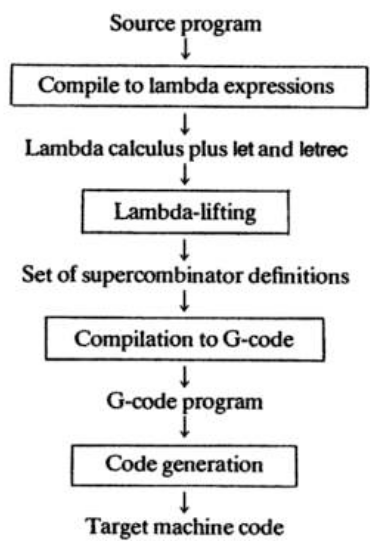
\includegraphics[scale=0.3]{gkomp.png}
\end{center}
\caption{Struktura G-kompajlera}
\label{fig:gcompiler}
\end{figure}
\fi 

\begin{primer}
	Predstavimo sad način na koji funkcioniše kompajler za G mašinu razmatrajući sledeću funkciju:
	\begin{center}
		\verb|f g x = K (g x)|.
	\end{center}
	Ova funkcija bi se prevela u sledeći niz instrukcija G-k\^ oda (svaka instrukcija je odvojena simbolom tačka-zapeta):
	\begin{center}
		\verb|Push 1|; \verb|Push 1|; \verb|Mkap|; \verb|Pushglobal K|; \verb|Mkap|; \verb|Slide 3|; \verb|Unwind|.
	\end{center}
\end{primer}
%referenca za primer i vise info o G masinama Implementing Functional Languages:a tutorial Simon L Peyton Jones Department of Computing Science, University of Glasgow and David R LesterDepartment of Computer Science, University of Manchesterc 1991

\begin{figure}[h!]
	\centering
	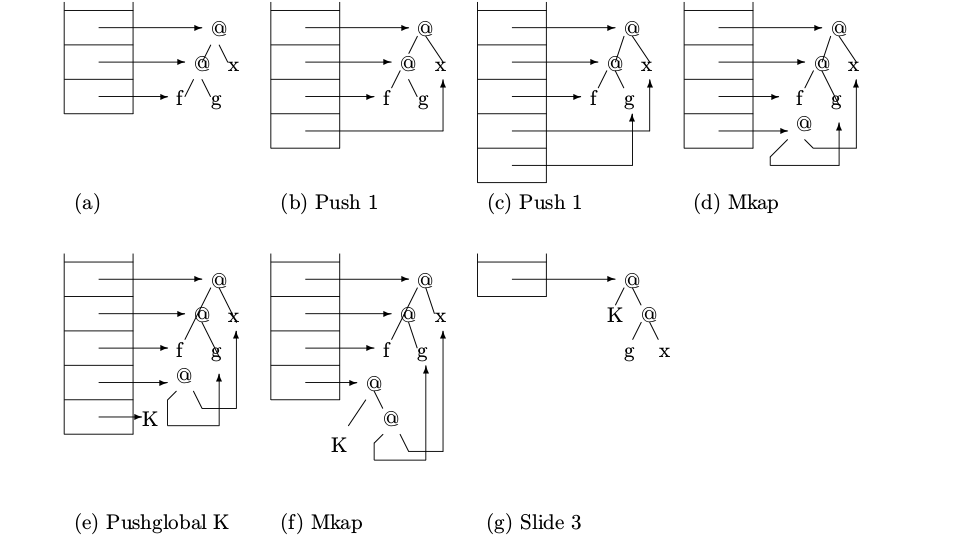
\includegraphics[scale=0.35]{primerGmasine.png}
	
	\caption{Vizuelni prikaz izvršavanja k\^ oda.}
	\label{fig:primerGmasine}
\end{figure}

Na slici \ref{fig:primerGmasine} prikazujemo kako se k\^ od izvršava. Sa leve strane svakog dijagrama prikazan je stek, koji raste nadole. Ostatak svakog dijagrama je hip. Aplikativni čvorovi predstavljeni su karakterom \verb|@|, izrazi malim slovima, a superkombinatori velikim slovima latinice. Takođe, prikazano je stanje mašine pre izvođenja instrukcija za \verb|f|. Dva elementa na vrhu steka su pokazivači na aplikativne čvorove, čije su desne strane izrazi koji će biti vezani za \verb|g| i \verb|x|. Instrukcija \verb|Push| koristi relativno adresiranje u odnosu na vrh steka. Ignorišući pokazivač na supekombinatorski čvor \verb|f|, prvi element na steku dobija broj \verb|0|, naredni \verb|1|, itd.

Naredni dijagram (b) pokazuje kako se stek izmenio nakon primene \verb|Push 1| instrukcije. Ona stavlja pokazivač na izraz \verb|x| na stek. Nakon jos jednog izvršavanja \verb|Push 1| instrukcije, imamo pokazivač na \verb|g| na vrhu steka i onda imamo ono što je prikazano na dijagramu (c). Dijagram (d) pokazuje šta se dešava kada se izvrši \verb|Mkap| instrukcija. Ona uzima dva pokazivača sa steka i pravi aplikativni čvor, ostavljajući pokazivač na rezultat na steku. Na dijagramu (e) izvršavamo \verb|Pushglobal K| instukciju koja stavlja pokazivač na \verb|K| superkombinator. Na dijagramu (f) vidimo da još jedna \verb|Mkap| instrukcija završava instanciranje tela \verb|f|. 

Sada možemo zameniti originalni izraz \verb|f g x| novoinstanciranim telom \verb|K(g x)|. U prvoj (ne lenjoj) verziji G-mašine, jednostavno pomerimo telo nadole za 3 mesta na steku pomoću instrukcije \verb|Slide 3| (dijagram (g)). Konačno, \verb|Unwind| instrukcija uzrokuje dalju evaluaciju.

%za sve ref dodati Abstract machines for programming language implementation Stephan Diehl a,∗, Pieter Hartel b, Peter Sestoft c a FB-14 Informatik, Universität des Saarlandes, Postfach 15 11 50, 66041 Saarbrücken, Germany b Department of Electronics and Computer Science, University of Southampton, Highfield, Southampton SO17 1BJ, UK c Department of Mathematics and Physics, Royal Veterinary and Agricultural University, Thorvaldsensvej 40,DK-1871 Frederiksberg C, Denmark Accepted 24 June 1999
